\section{Introduction}
DESY (Deutsches Elektronen-Synchrotron) is one of very few research institutes 
world wide that provides test beams with energies up to 6.3\,GeV. By adjusting 
some parameters for the test beam generation, the test beam users can vary the 
energy and rate of the three independent test beam lines as needed. Therefore, 
the particle energy can range between 1\,GeV and 6.3\,GeV, and the rate between 
1\,Hz and far beyond 10\,kHz.\\The test beam lines originate at the DESY-II 
synchrotron ring, which accelerates a single bunch of about 10$^{10}$ 
electrons/positrons per time to an energy of 6.3\,GeV. The beam bunch hits a 
primary target that is positioned in the beam pipe at the origin of the test 
beam line. Bremsstrahlung photons are emitted and hit a converter plate, where 
they are converted into electron/positron pairs due to pair production. The 
electron/positron beam continues along the test beam line and enters a dipole 
magnet. Because of the energy distribution and opposite charge of the electrons 
and positrons, the beam is widened into a particle fan in the magnetic field of 
the dipole magnet. The particles leaving the magnet are then collimated by a 
collimator positioned behind the magnet. The users can select the energy of the 
final beam by adjusting the current through the magnet and therefore the 
particle deflection. By varying the deflection radius, a different part of the 
electron/positron fan enters the test beam area, where the users' experimental 
set-up is placed. The components of the whole test beam generation are 
schematically shown in Figure~\ref{fig:Testbeam scheme}.

\begin{figure}[ht]
  \centering
  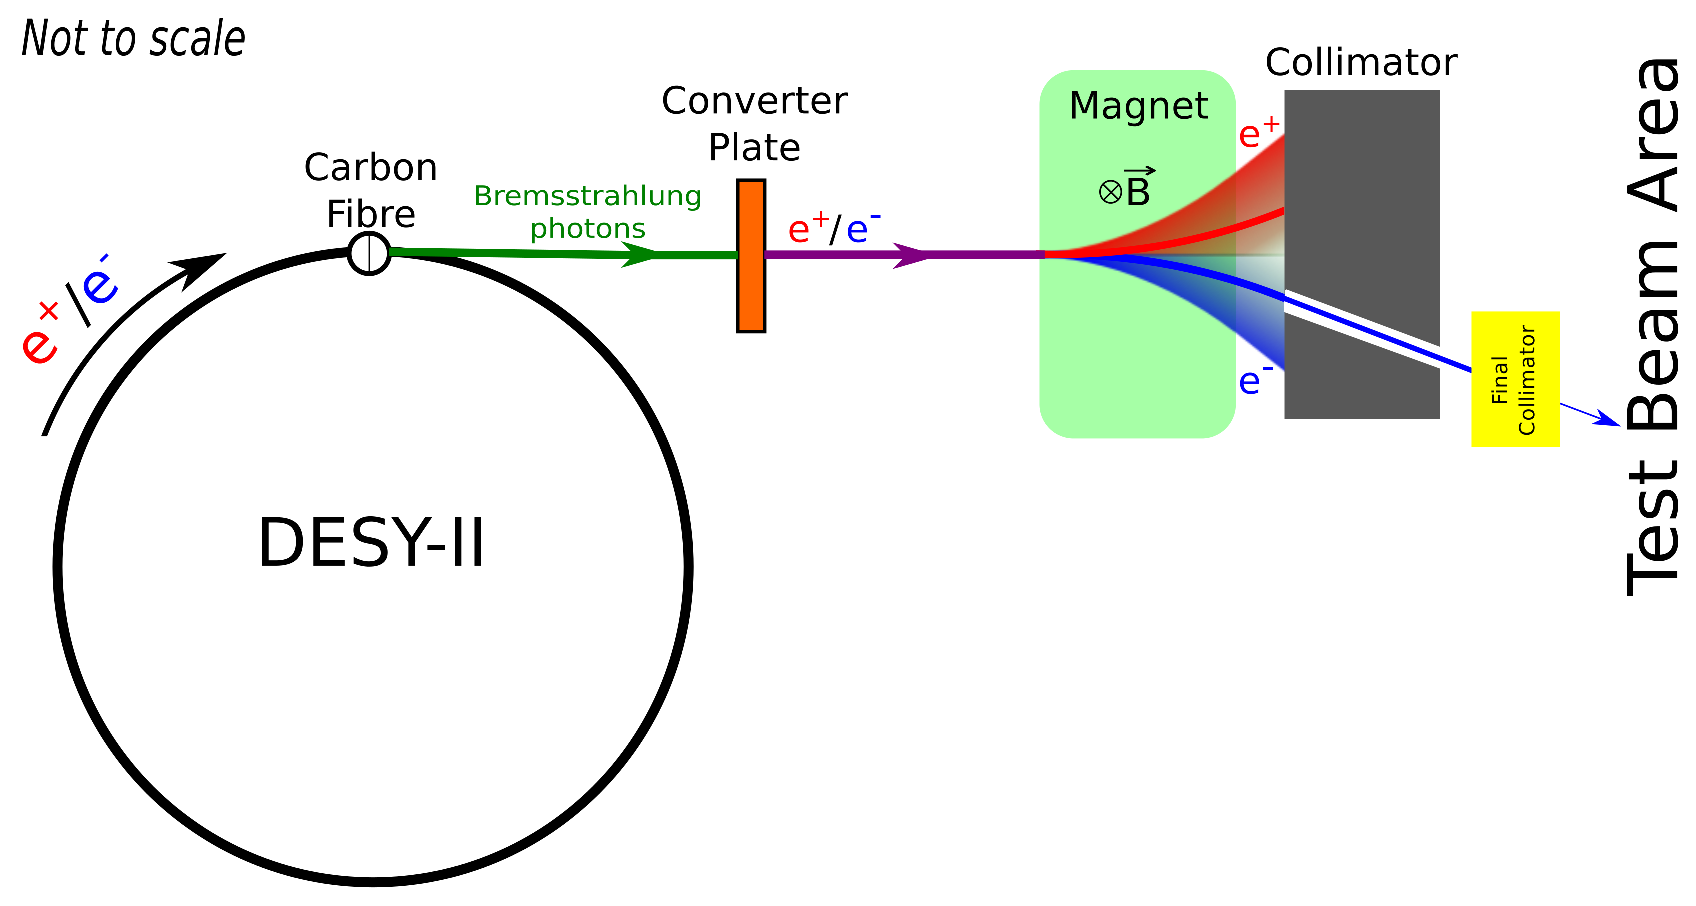
\includegraphics[width=0.775\textwidth]{DESYII-Schematic_new.eps}
  \caption[Scheme of the test beam generation.]{A scheme of the beam generation in the DESY-II Test Beam Facility.}
    \label{fig:Testbeam scheme}
\end{figure}

The test beam line components were simulated to study the energy distributions 
of the test beams along their generation and to provide a full simulation 
toolkit of the DESY-II test beam lines. The toolkit allows easily to change or 
add beam generation components in the geometry description for the test beam 
simulation, so that with the help of the simulated data deeper understanding is 
gained about the beam attributes for all possible settings: the particle fluxes 
in the accelerator tunnel, the beam energy distributions, and the beam rate for 
the final electron/positron beam.\\At the same time, the information from the 
simulation serves as the key input for future test beam line improvements, as 
well as for the optimisation of the test beam users' experimental set-up. The 
simulation data can be used as an input for other Monte Carlo simulations and 
studies, and will allow even more accurate simulation/data comparisons of sensor 
tests and other experiments for the particle detector development.